\section{Experimental results}

\subsection{Basic results}\label{basicResults}

We present in Figure \ref{fig:basicResults} the results of executing the TPC-DS benchmark at the 1 TB scale factor on the SUTs under consideration using the hardware and software configuration described in the previous section. The total time is divided into the three benchmark tests, namely the data loading, power, and throughput tests.

\begin{figure}
   \begin{center}
   \scalebox{0.80}{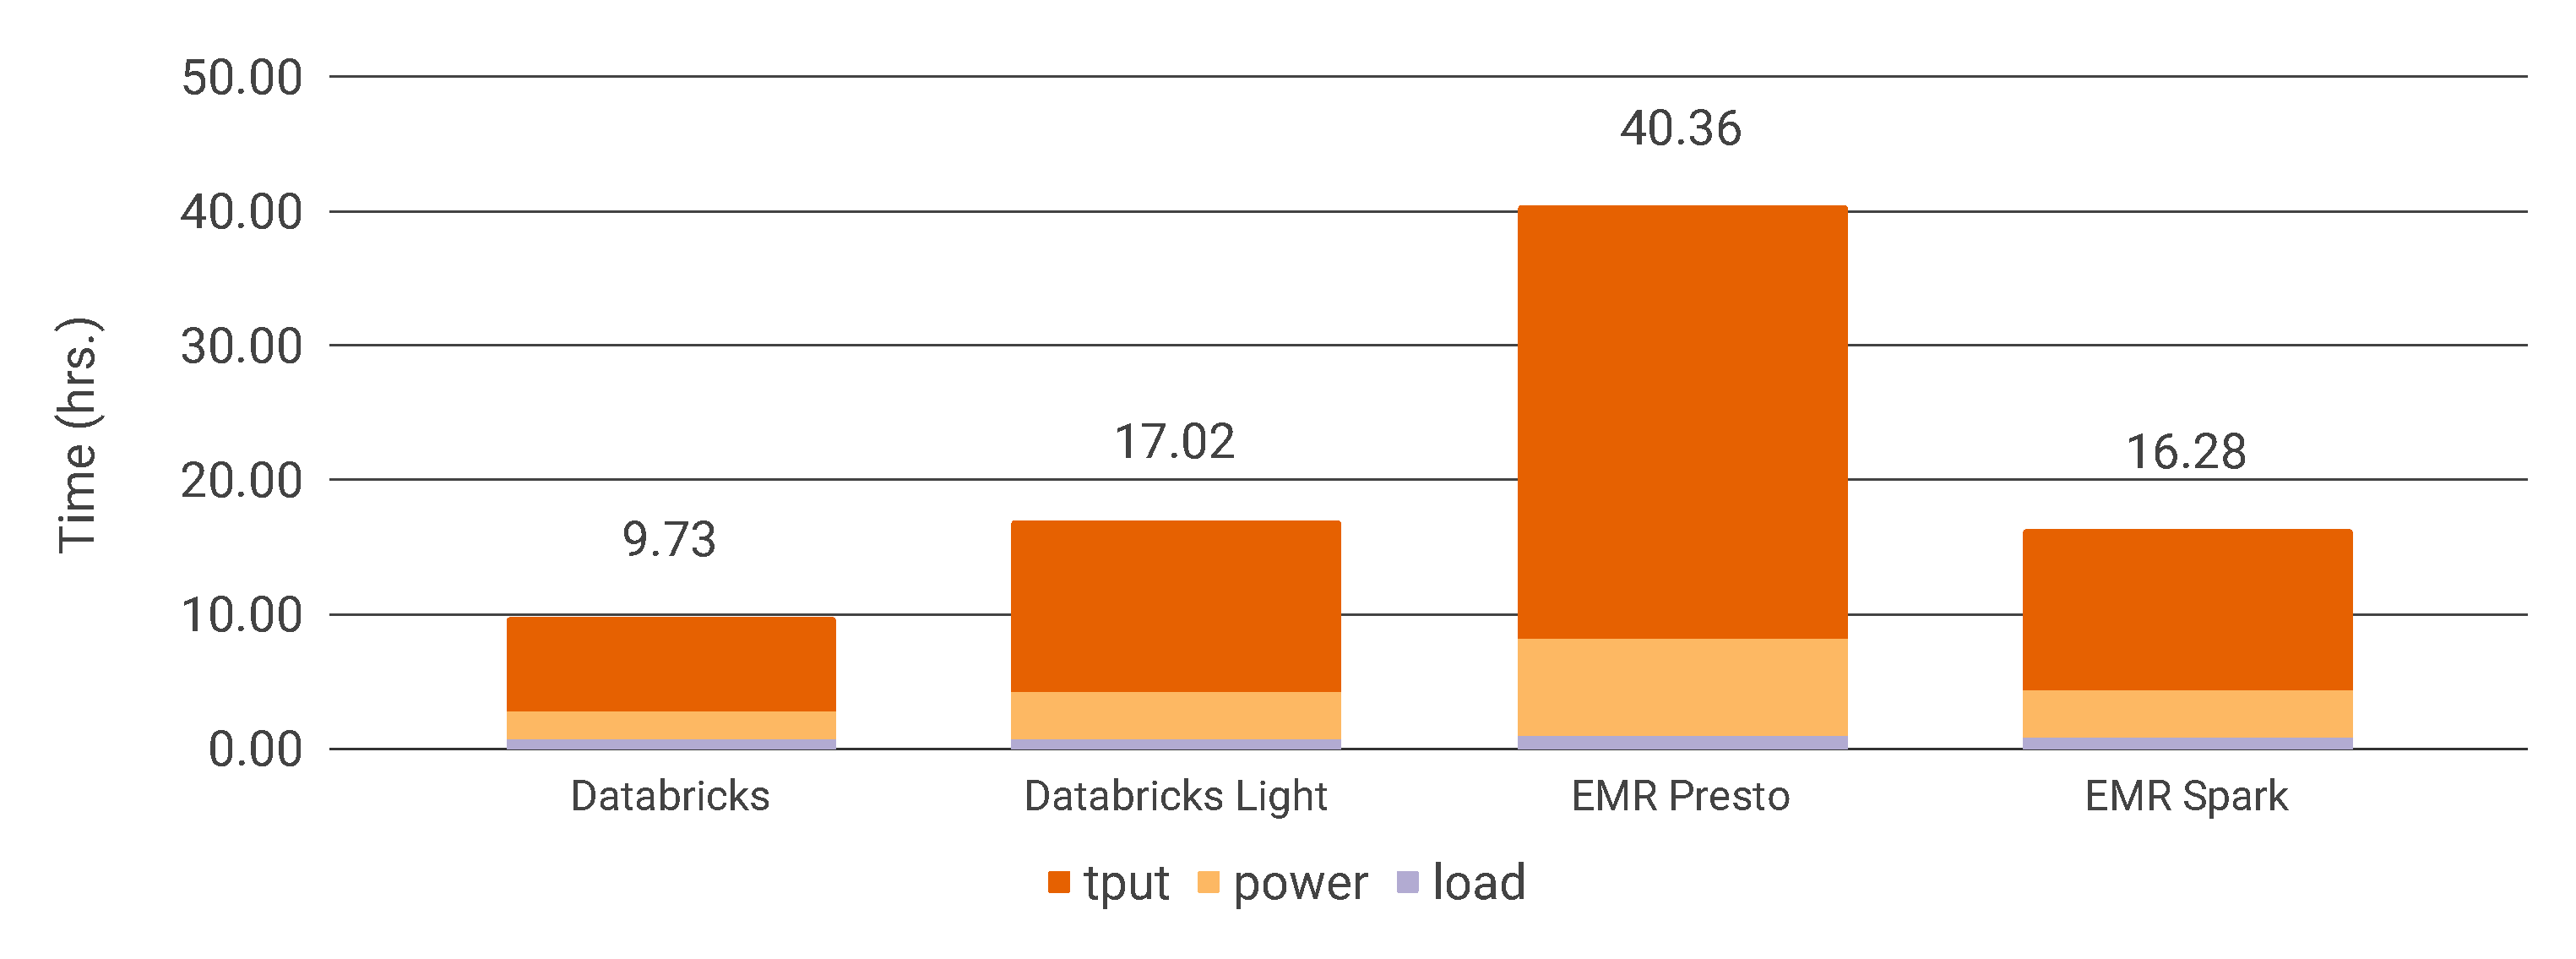
\includegraphics[width=7.0in]{imgs/basicResults.pdf}}
   \end{center}
   \caption{Basic results for the TPC-DS benchmark at the 1 TB scale factor.}
   \label{fig:basicResults}
\end{figure}

In order to load the data, we first generate raw text files in CSV format by means of the data generator included in the TPC-DS Toolkit. These files are stored in an AWS S3 bucket and processed by the various systems to generate database table files in columnar storage formats. Concretely, we use Apache Parquet for Databricks and EMR Spark, while for EMR Presto we opted for Apache ORC since early tests showed it to be more efficient. The database table files are stored in S3 buckets and accessed by the SUTs cluster machines located in the same AWS region (us-west-2). In all cases, as shown in Figure \ref{fig:basicResults}, the data loading time is less than one hour and represents a very small fraction of the total benchmark execution time.

The Power and Throughput Tests are then run on the loaded data, completing the benchmark execution. Recall that the Power Test involves running all 99 queries individually in sequence, while the Throughput Test runs a series of query streams (i.e. predefined permutations of the original query sequence) concurrently. In our case we run 4 query streams, adding up to a total of 396 queries.

The results of Figure \ref{fig:basicResults} show that Databricks obtains the best result by completing the benchmark in slightly less than 10 hours, which is more than 4 times faster than EMR Presto, the slowest system overall. EMR Spark is faster than its Presto counterpart, but it still takes over 16 hours, yielding the second-best time. With a time of almost exactly 17 hours, Databricks Light ranks third in total benchmark completion time.

\subsection{Results with table and column statistics}\label{statsResults}

We can improve the results shown in the previous subsection and characterized as basic by collecting statistics on the data that will allow the cost-based query optimizer (CBO) of each system to generate optimized evaluation plans. The statistics considered are collected at the table and column levels. The table-level statistics correspond to table size metrics such as the number of tuples or the disk space occupied. On the other hand, column-level statistics involve computing for a given column metrics including the number of distinct values, the minimum and maximum value, and the number or proportion of null values.

In our experiments, we produce statistics for all tables and all columns of each table. A secondary Analyze phase is added to the Data Loading Test for this purpose, and the time required is measured separately from the data loading process described earlier. The use of table and column statistics produces a new set of results summarized in Figure \ref{fig:statsResults}, which when ranked show the same order as the basic results. We also can see that the time required for statistics collection is comparatively negligible. 

\begin{figure}
   \begin{center}
   \scalebox{0.80}{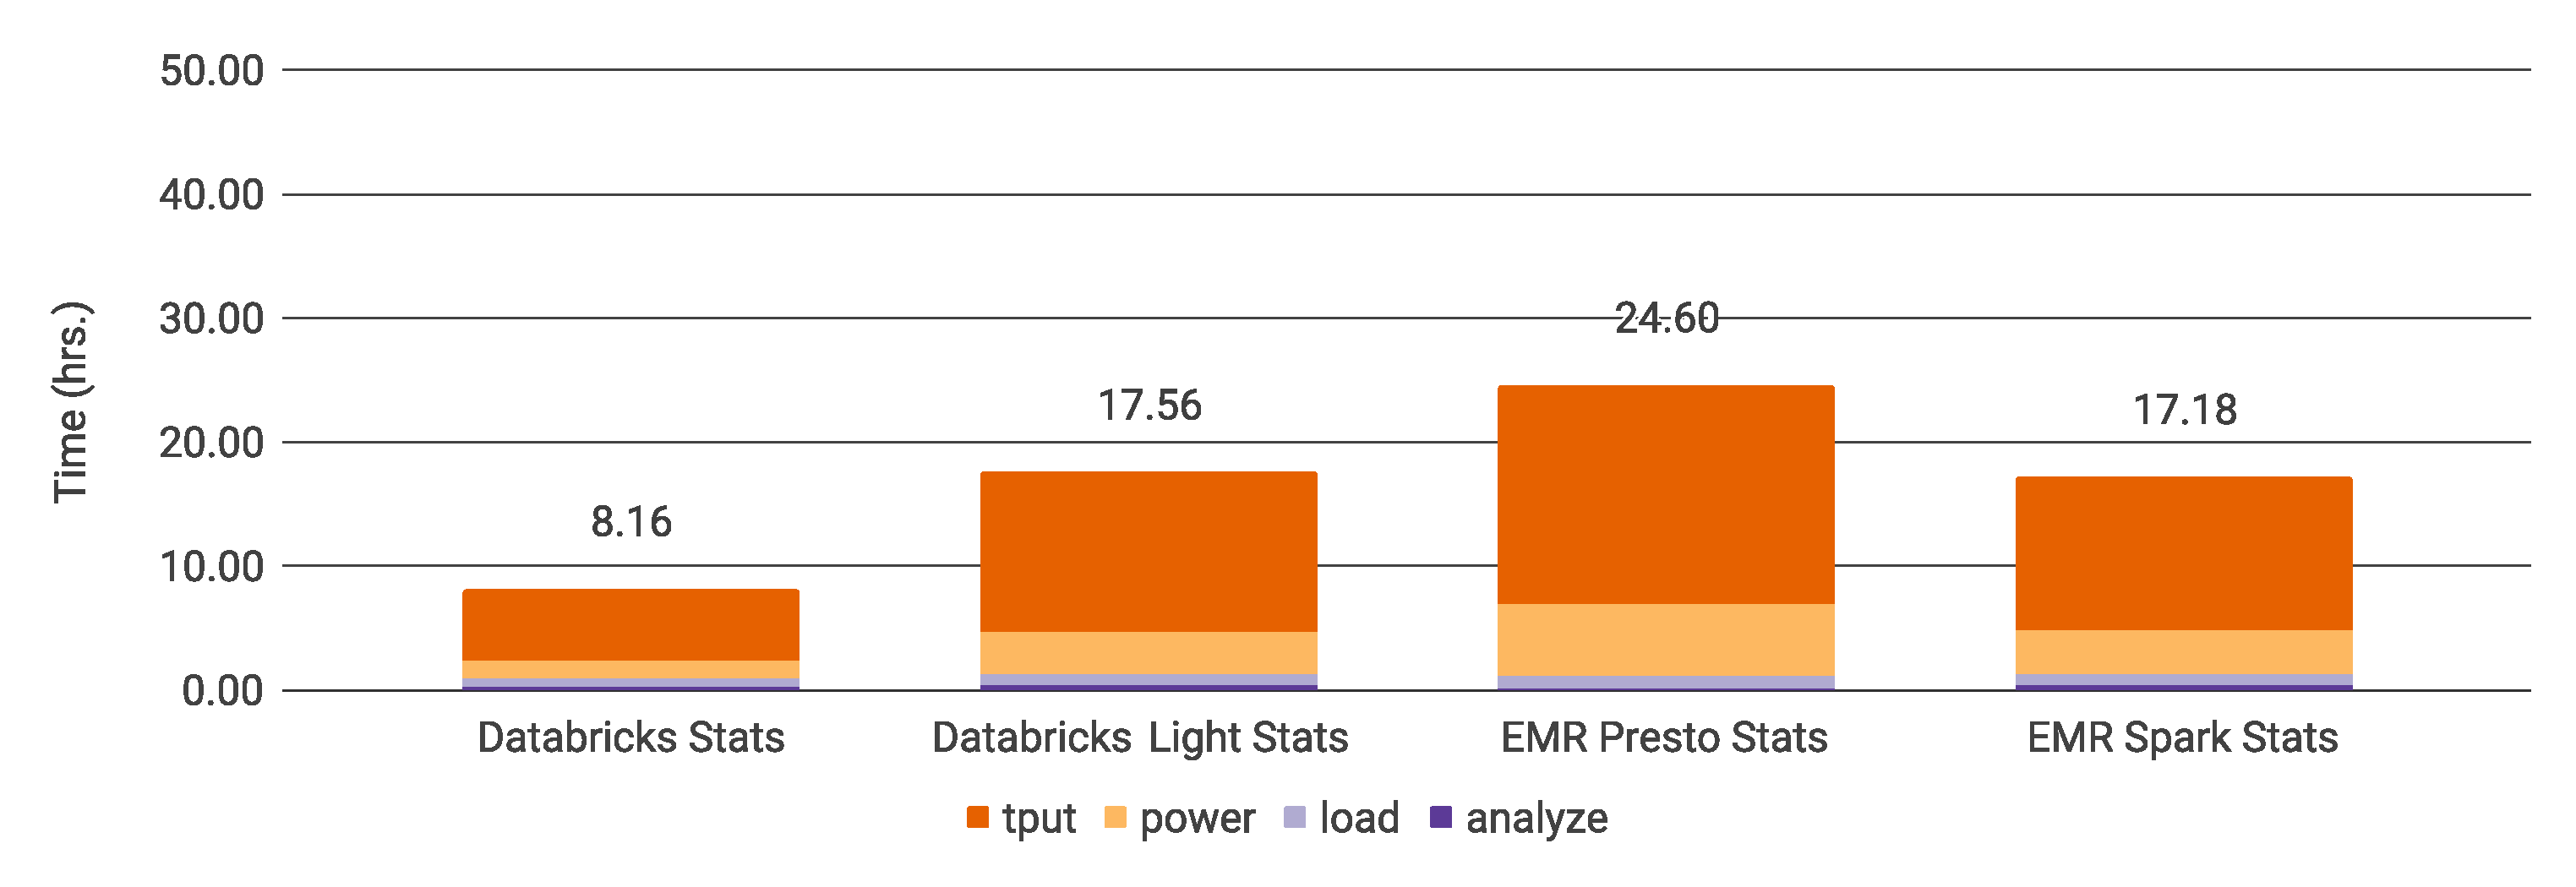
\includegraphics[width=7.0in]{imgs/statsResults.pdf}}
   \end{center}
   \caption{Results using table and column statistics for the TPC-DS benchmark at the 1 TB scale factor.}
   \label{fig:statsResults}
\end{figure}

In order to study in greater detail the effect of employing statistics, besides comparing the summarized results using statistics in Figure \ref{fig:statsResults} with the basic results from Figure \ref{fig:basicResults}, we can calculate the speedup (ratio between the two times) for each system. Figure \ref{fig:statsSpeedup} shows the speedup achieved with table and column statistics.

\begin{figure}
   \begin{center}
   \scalebox{0.70}{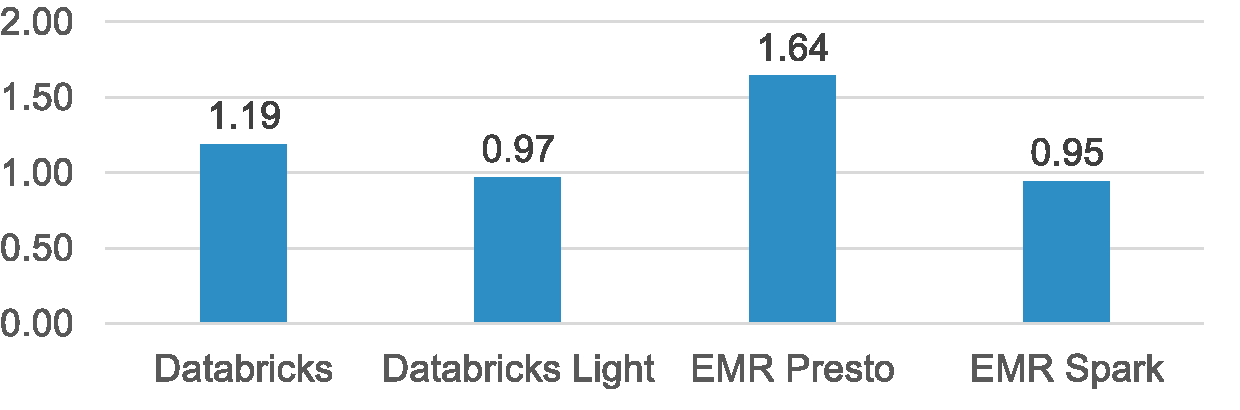
\includegraphics[width=7.0in]{imgs/statsSpeedup.pdf}}
   \end{center}
   \caption{Speedup using table and column statistics for the TPC-DS benchmark at the 1 TB scale factor.}
   \label{fig:statsSpeedup}
\end{figure}

We observe the biggest speedup with EMR Presto at 1.64, followed by Databricks at 1.19. Databricks is thus about 3 times faster than EMR Presto when using statistics in contrast to about 4 times faster with the basic results. This does not necessarily imply that the EMR Presto optimizer is more effective, since the evaluation strategies for the EMR Presto basic results could be significantly suboptimal from the start.

Notably, Databricks Light and EMR Spark show reduced performance when using statistics, reflected in speedups of less than 1. In the case of EMR Spark it is important to clarify that the result in Figure \ref{fig:statsResults} was obtained with the default configuration in which the optimizer is disabled. With the optimizer enabled the total benchmark execution time rises from 17.28 hours to 27.11 hours, which corresponds to a speedup of 0.60.








